\documentclass[
t, % align text inside frame to t=top, b=bottom, c=center
10pt, % 8pt, 9pt, 10pt, 11pt, 12pt, 14pt, 17pt, 20pt available as text font
aspectratio=1610, % select your aspect ratio 4:3=43, 16:9=169, 16:10=1610
ngerman,
english,
%handout,
]{beamer}
\usetheme{Juelich}

\usepackage{babel}
\usepackage[utf8]{inputenc}
\usepackage[labelfont=bf]{caption}
\usepackage[colorlinks=true, urlcolor=blue]{hyperref}
\usepackage{pdfpages}

\title{Introduction to Version Control}
\subtitle{Time travel for beginners}
\author{Julia Sprenger}
\institute[My Institute]{INM-6/10}
\date{June 29, 2018}
\titlegraphic{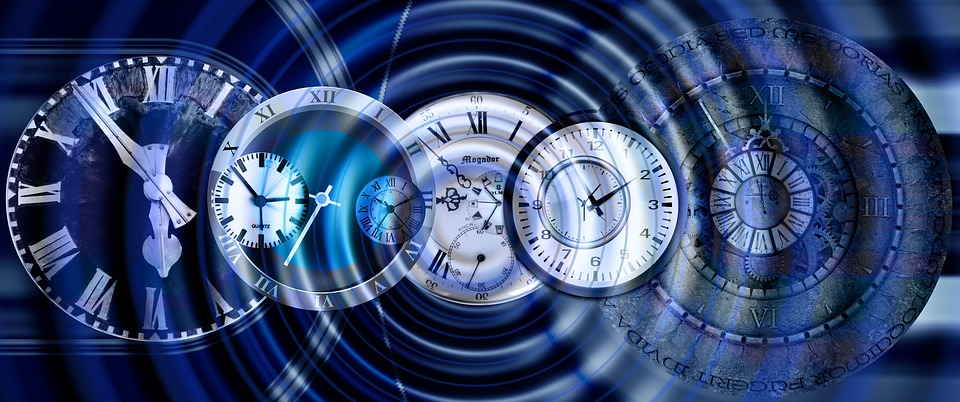
\includegraphics[width=\paperwidth]{graphics/clock-1527693_960_720.jpg}}

\newcommand\blfootnote[1]{%
  \begingroup
  \renewcommand\thefootnote{}\footnote{#1}%
  \addtocounter{footnote}{-1}%
  \endgroup
}

\begin{document}
% only use \maketitle to set your titlepage
\fzjset{title page=image}
\maketitle

% \fzjset{title page=text}
% \maketitle

\part{Why should I care about versions?}
\makepart

\begin{frame}
    \centering
    
\includegraphics[height=\textheight]{graphics/phd101212s.jpg}\\
    \url{http://phdcomics.com/comics.php?f=1531}
\end{frame}

\begin{frame}
    \centering
    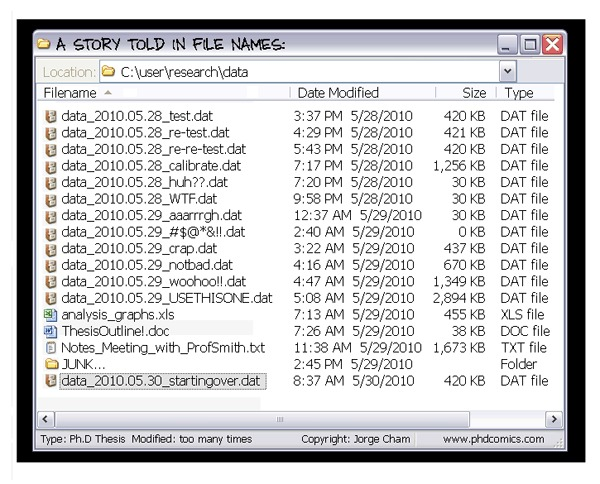
\includegraphics[height=\textheight]{graphics/phd052810s.jpg}\\
    \url{http://phdcomics.com/comics.php?f=1323}
\end{frame}

\begin{frame}
    \frametitle{Version Control using folder and filenames}
    \begin{itemize}[<+->]
        \item only readable by you ...
        \item ... as long as you remember
        \item no consistent structure or naming scheme enforced
        \item no detailed description of changes (why were changes performed?)
        \item no easy way of comparing changes between versions (which changes were performed?)
        \item \dots{}
    \end{itemize}
\end{frame}

\begin{frame}
    
\includepdf[pages=9, offset=0mm 10mm, scale=0.9]{sources/git-github.pdf}
    \blfootnote{\url{https://github.com/rstudio/webinars/tree/master/06-Collaboration-and-time-travel-version-control}}
\end{frame}

\begin{frame}
    
\includepdf[pages=10, offset=0mm 10mm, scale=0.9]{sources/git-github.pdf}
    \blfootnote{\url{https://github.com/rstudio/webinars/tree/master/06-Collaboration-and-time-travel-version-control}}
\end{frame}

\part{Version Control Systems}
\makepart

\begin{frame}
    \frametitle{Different Version Control Systems}
    \centering
    \vfill
    \begin{tabular}{ c l r }
        
\includegraphics[height=0.8cm]{graphics/giticon_orange.eps} & \large{GIT} &  distributed system\\
        
\includegraphics[height=0.8cm]{graphics/Mercurial_logo.png} & \large{Mercurial} &  distributed system\\
        
\includegraphics[height=0.8cm]{graphics/Subversion_Logo.png} & \large{SVN} &  centralized system\\
    \end{tabular}
    \vfill
\end{frame}

\section{GIT}
\begin{frame}
    \frametitle{GIT}
    \blfootnote{\url{https://github.com/rstudio/webinars/tree/master/06-Collaboration-and-time-travel-version-control}}
    \begin{minipage}{0.5\textwidth}
	\begin{itemize}
	    \item only selected version present on disc
	    \item history stored in hidden .git folder
	    \item smart version handling for text based files by using file differences
	\end{itemize}
    \end{minipage}
    \hfill
    \begin{minipage}{0.5\textwidth}
	
\includepdf[pages=12, width=0.6\textwidth, offset=20mm 0mm,]{sources/git-github.pdf}
    \end{minipage}
\end{frame}

\begin{frame}
    \frametitle{GIT}
    
\includepdf[pages=13, offset=0mm 10mm, scale=0.9]{sources/git-github.pdf}
    \blfootnote{\url{https://github.com/rstudio/webinars/tree/master/06-Collaboration-and-time-travel-version-control}}
\end{frame}
\begin{frame}
    \frametitle{GIT}
    
\includepdf[pages=14, offset=0mm 10mm, scale=0.9]{sources/git-github.pdf}
    \blfootnote{\url{https://github.com/rstudio/webinars/tree/master/06-Collaboration-and-time-travel-version-control}}
\end{frame}
\begin{frame}
    \frametitle{GIT}
    
\includepdf[pages=15, offset=0mm 10mm, scale=0.9]{sources/git-github.pdf}
    \blfootnote{\url{https://github.com/rstudio/webinars/tree/master/06-Collaboration-and-time-travel-version-control}}
\end{frame}
\begin{frame}
    \frametitle{GIT}
    
\includepdf[pages=16, offset=0mm 10mm, scale=0.9]{sources/git-github.pdf}
    \blfootnote{\url{https://github.com/rstudio/webinars/tree/master/06-Collaboration-and-time-travel-version-control}}
\end{frame}

\begin{frame}
    \frametitle{GIT Interfaces}
    \centering
    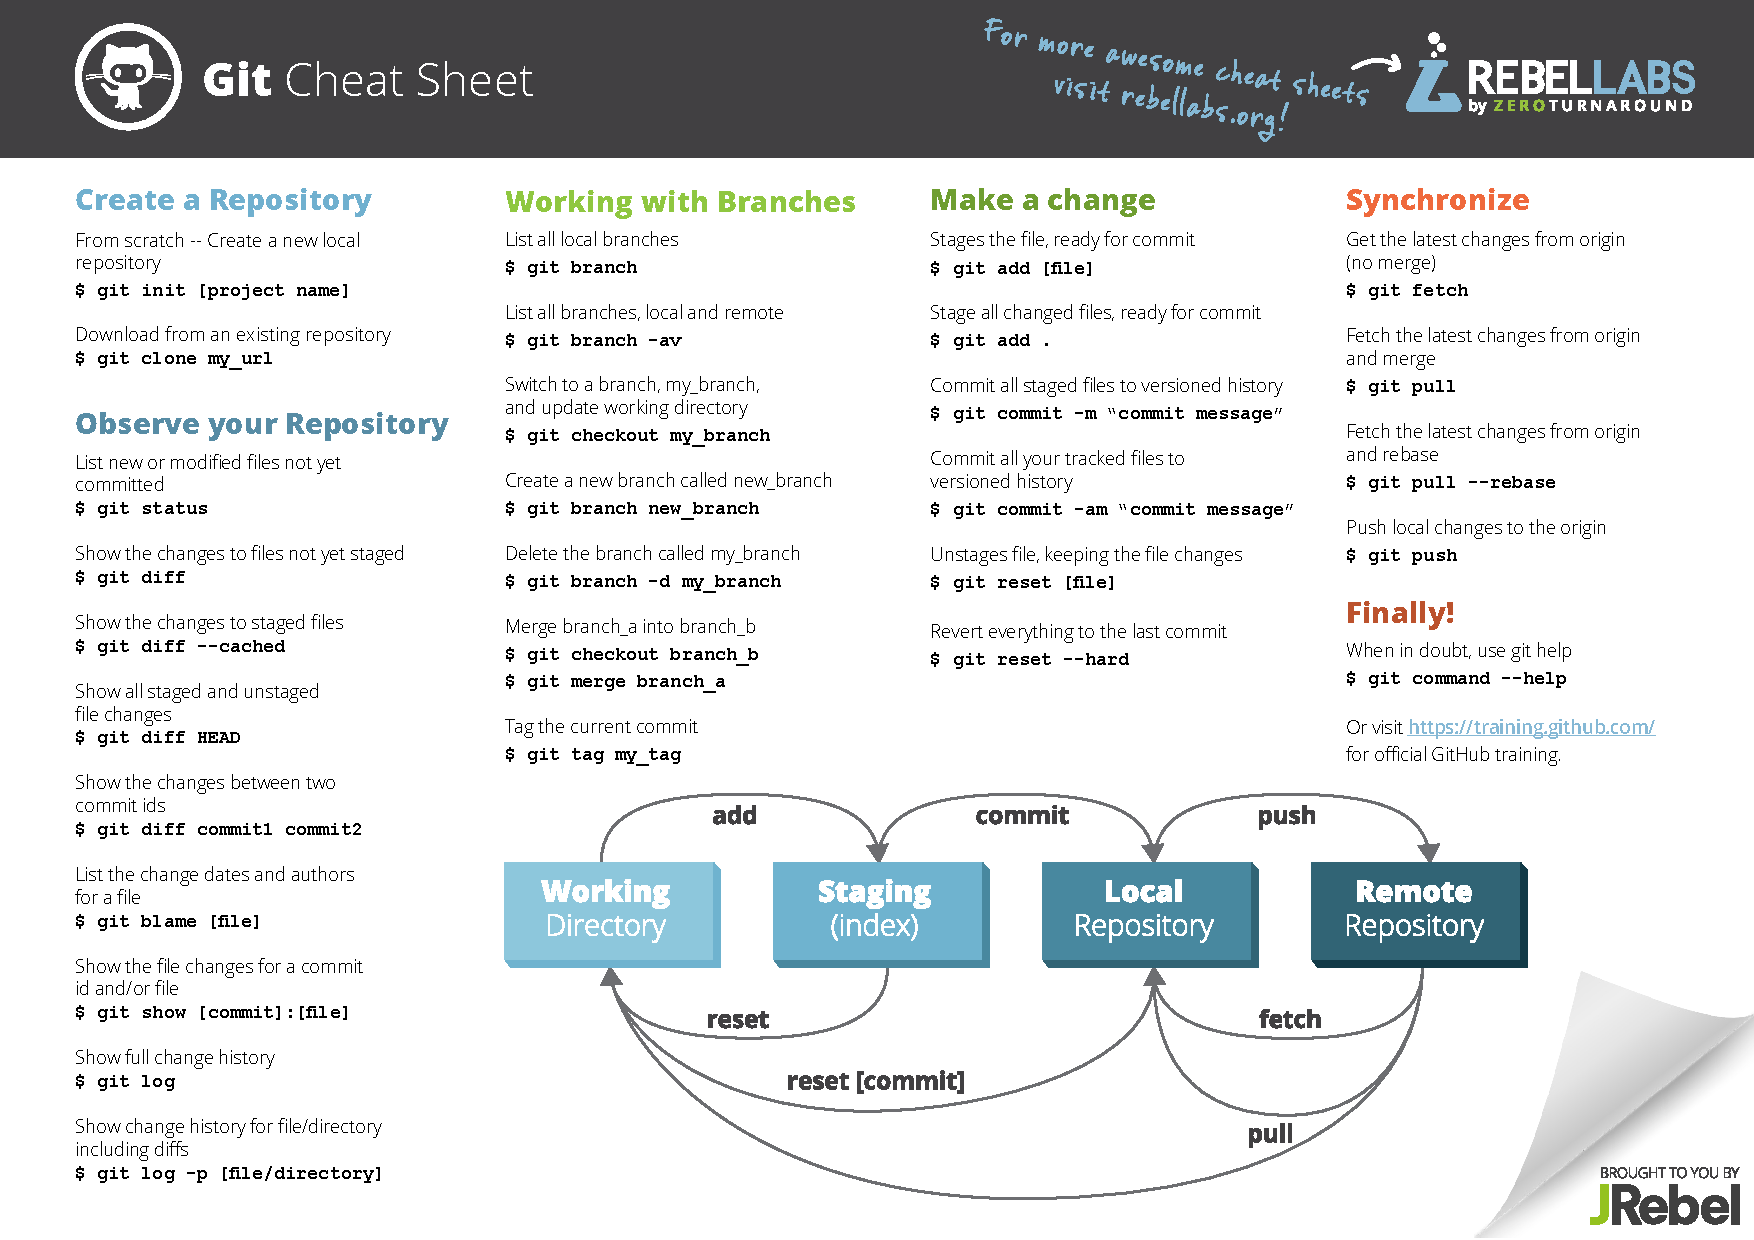
\includegraphics[height=0.8\textheight]{graphics/zt_git_cheat_sheet.pdf}\\
    \blfootnote{\url{http://files.zeroturnaround.com/pdf/zt_git_cheat_sheet.pdf}}
\end{frame}

\begin{frame}
    \frametitle{GIT Interfaces}
    \centering
    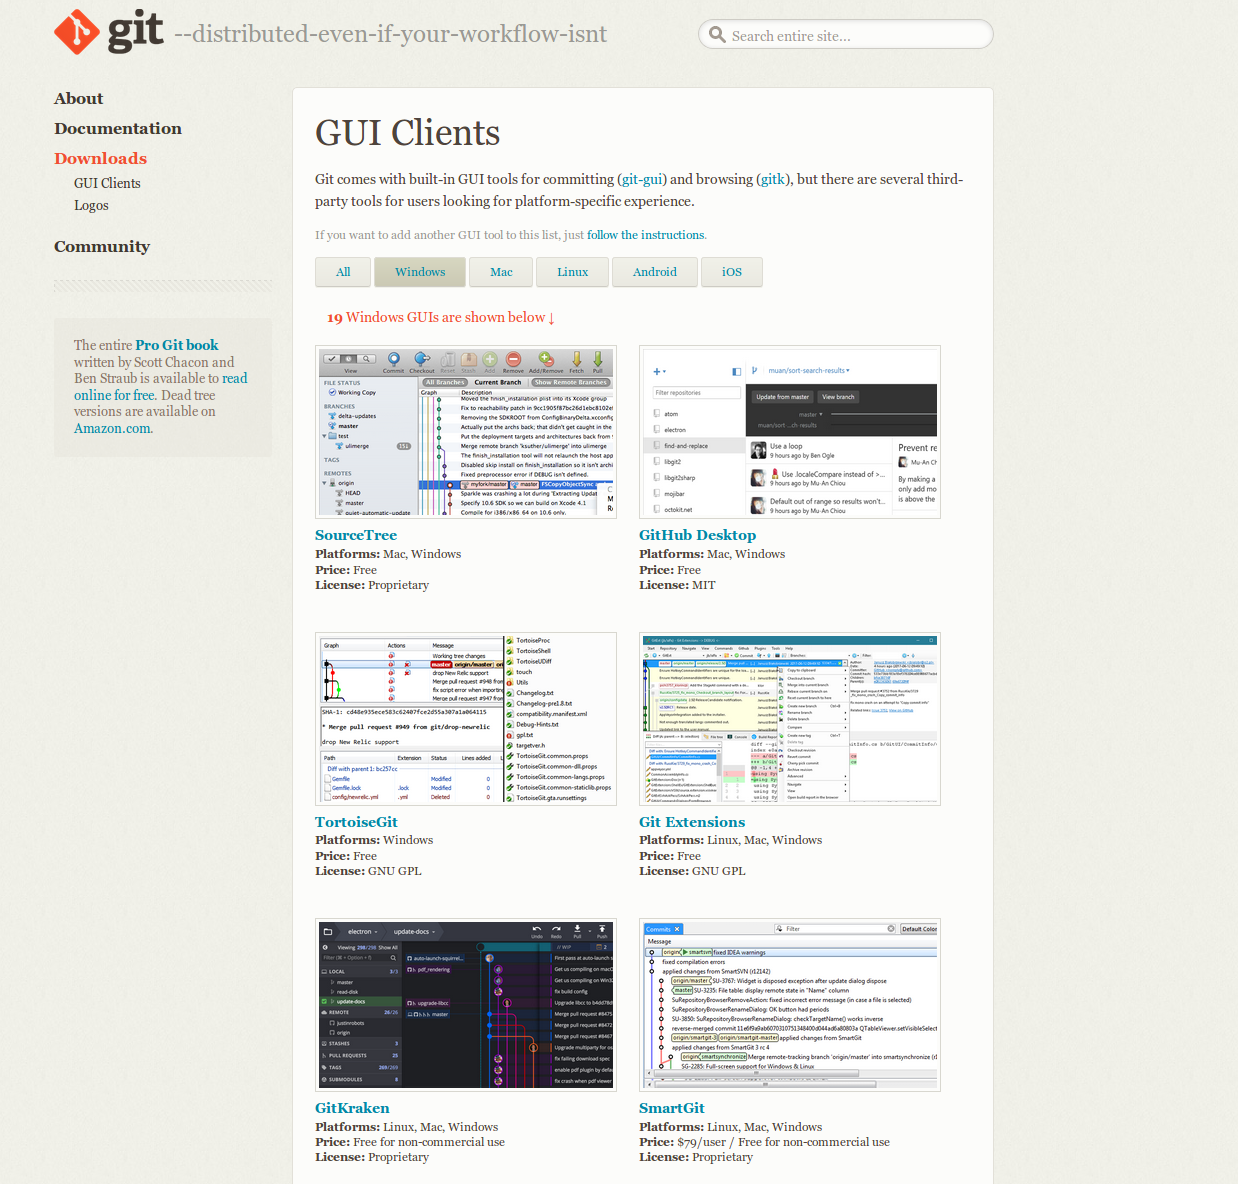
\includegraphics[height=0.8\textheight]{graphics/Screenshot_GUI_Clients.png}\\
    \blfootnote{\url{https://git-scm.com/download/gui}}
\end{frame}

\begin{frame}
    \frametitle{GIT Interfaces}
    \centering
    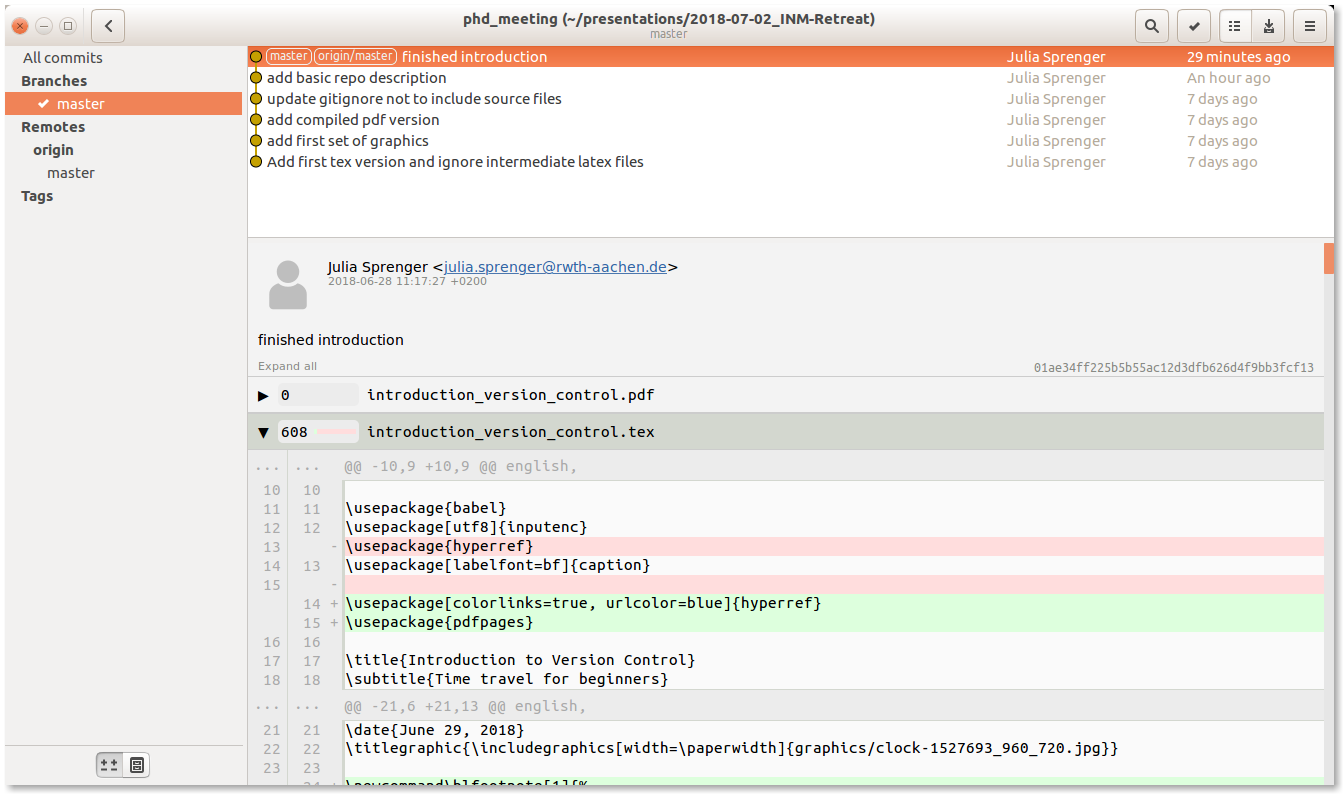
\includegraphics[height=0.8\textheight]{graphics/Screenshot_gitg.png}\\
\end{frame}

\part{Collective Version Control}
\makepart

\begin{frame}
    \frametitle{Collaborative Chaos Control}
    \centering
    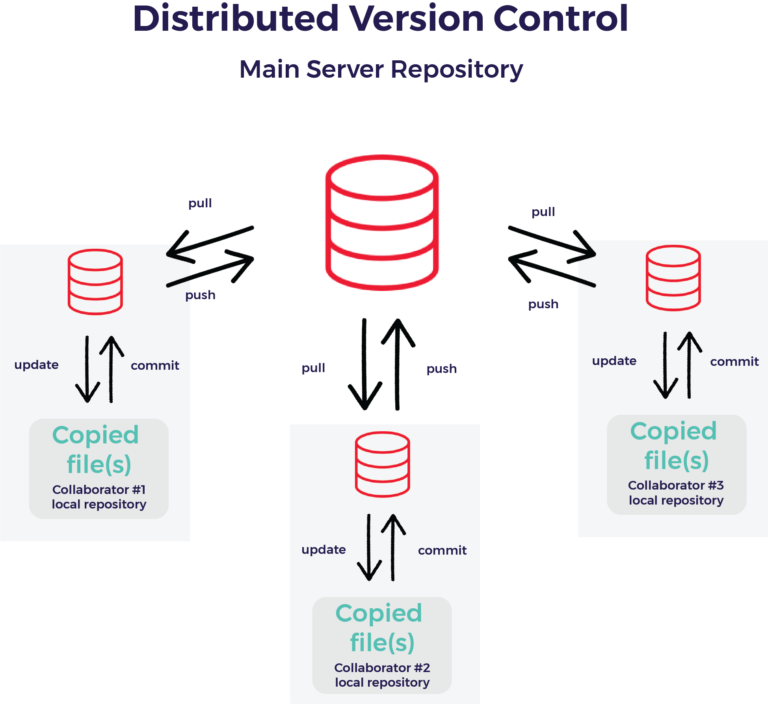
\includegraphics[height=0.7\textheight]{graphics/DVC-distributed-version-control-768x704.png}\\
    \url{https://www.positivethinkingcompany.com/articles/articles-web-mobile/git-technology-simplifies-coding-collaboration/}
\end{frame}

\begin{frame}
    \frametitle{Collaborative Chaos Control}
    \centering
    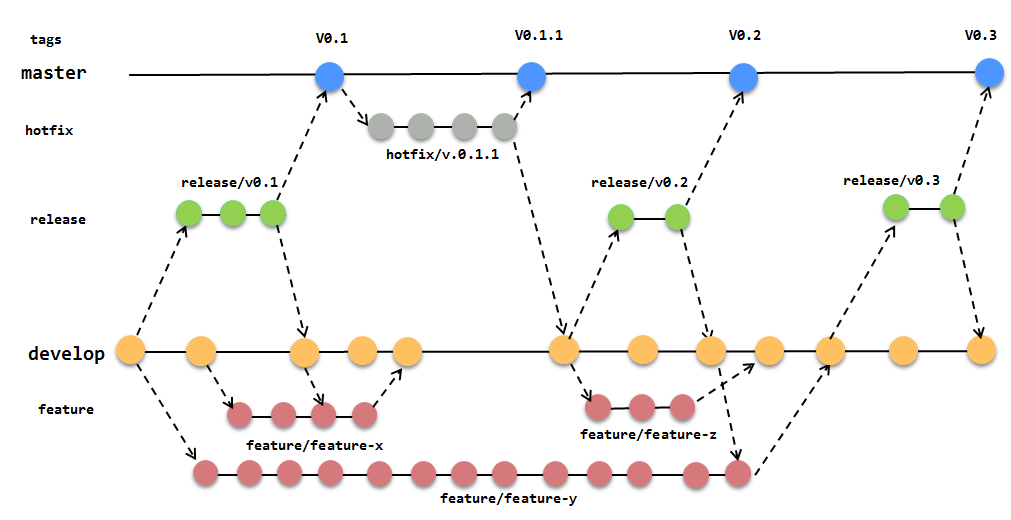
\includegraphics[height=0.7\textheight]{graphics/gitflow.png}\\
    \url{https://fpy.cz/pub/slides/git-workshop}
\end{frame}


\begin{frame}
    \frametitle{GitHub}
    \begin{columns}
          \column{0.58\linewidth}
             \centering
             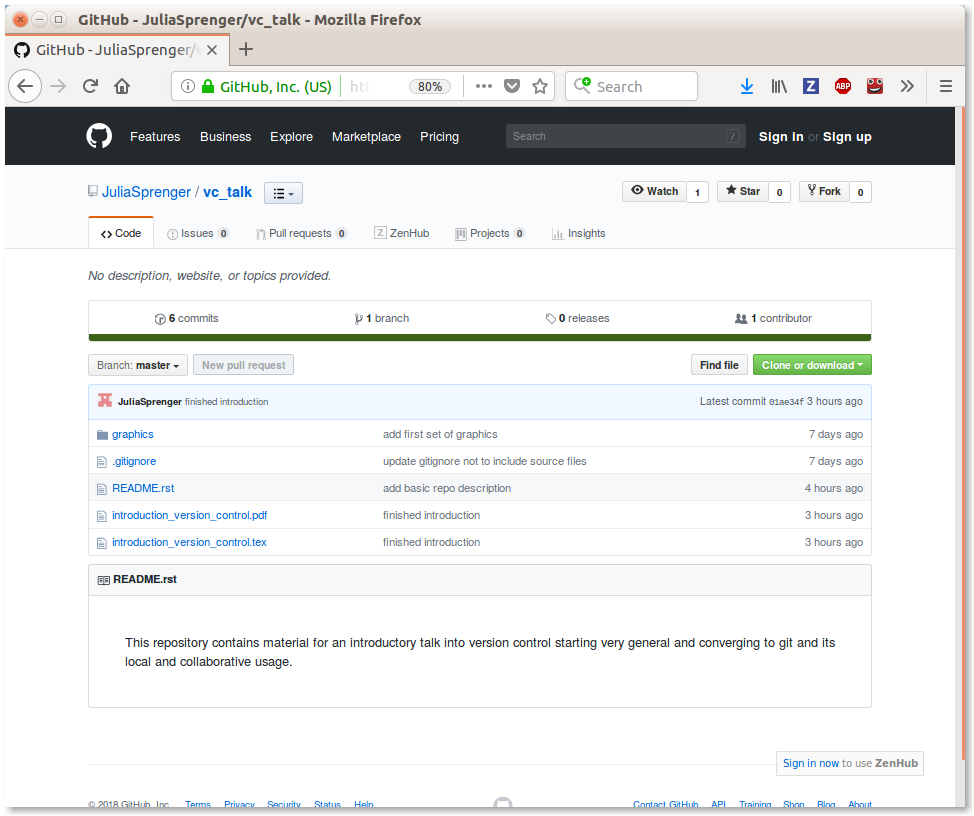
\includegraphics[width=\textwidth]{graphics/Screenshot_github}
           \column{0.38\linewidth}
	      \vspace{-5cm}
	      \begin{itemize}
		  \item visualization of repository content and changes
		  \item issue collection \& discussion
		  \item pull requests
		  \item statistics
		  \item \textbf{public} \& private repositories
	      \end{itemize}
         \end{columns} 
    \end{frame}
\end{frame}

\begin{frame}
    \frametitle{GIN}
    \centering
    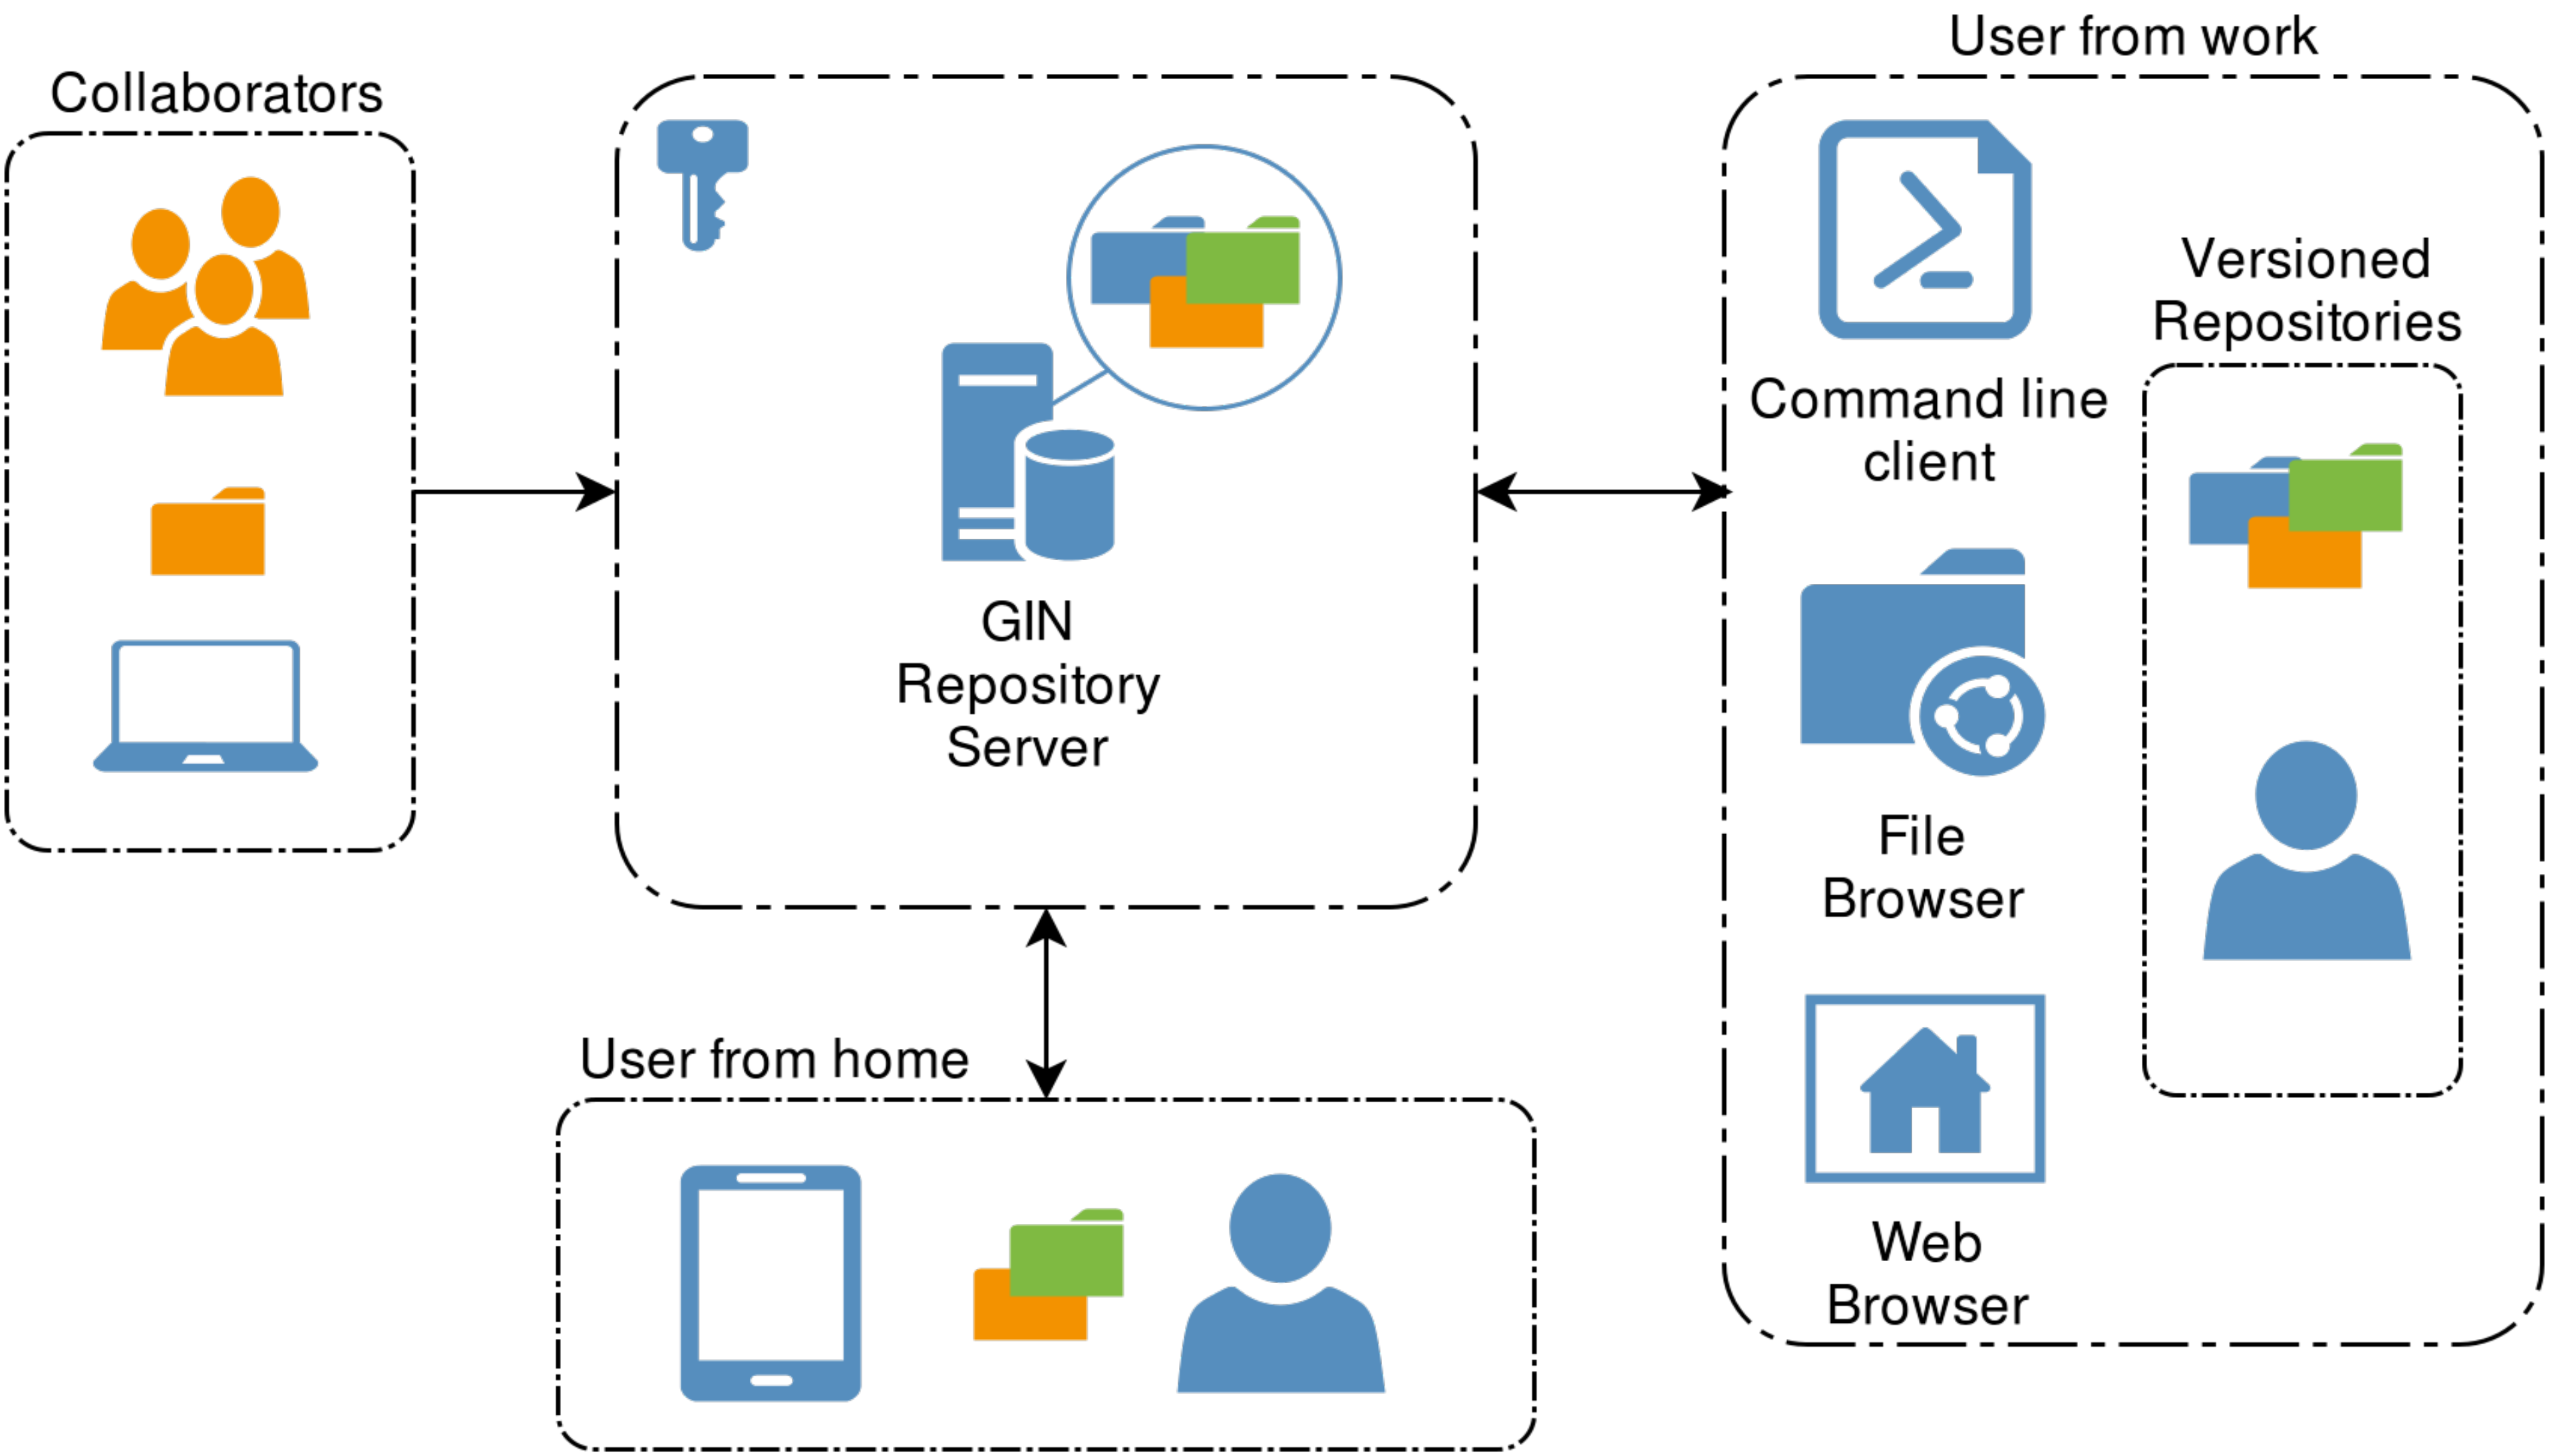
\includegraphics[height=0.7\textheight]{graphics/image9539.png}\\
\end{frame}

\part{Version Control for 'big data'}
\makepart

\begin{frame}
    \frametitle{GIT-ANNEX \& GIN}
    \begin{columns}
        \column{0.4\linewidth}
	
\includegraphics[height=1cm]{graphics/gitannex_logo}\textbf{GIT-ANNEX}\\
	\url{https://git-annex.branchable.com}\\
	\begin{itemize}
	    \item better suited for large and binary files
	    \item large files are only copied when necessary
	    \item large files are only downloaded by request
	\end{itemize}
	\column{0.4\linewidth}
	
\includegraphics[height=1cm]{graphics/GinLogo}\\
	\url{https://web.gin.g-node.org}\\
	\begin{itemize}
	    \item data management service based on git and git-annex
	    \item public \& private repositories
	    \item DOI service
	    \item version controlled
	    \item open source
	    \item developed and hostet by German Neuroinformatics Node
	\end{itemize}
    \end{columns}\\
\end{frame}


\section{Summary}

\begin{frame}
    \frametitle{Summary}
    \begin{itemize}
	\item Version control can help manage your files for
	\begin{itemize}
	    \item local projects
	    \item collaborative projects via GitHub
	\end{itemize}
	\item GIT is a distributed version control system ideal for text based files
	\item GIT-ANNEX extends GIT functionality to also cover large, binary files
	\item GIN is a data management platform using GIT and GIT-ANNEX
    \end{itemize}
    \centering
    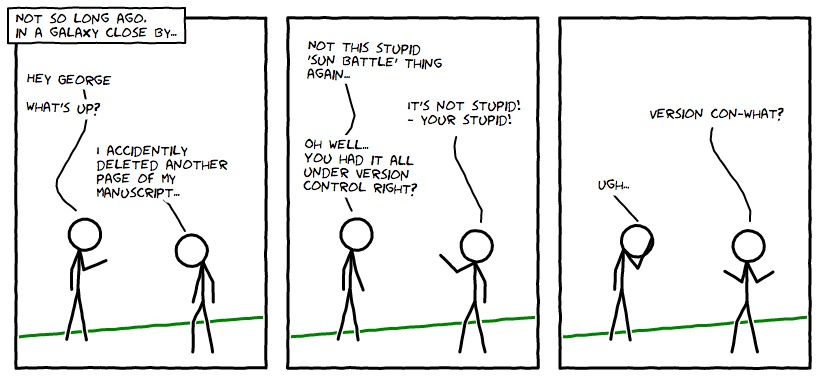
\includegraphics[height=0.55\textheight]{graphics/vc-xkcd.jpg}
    \url{http://smutch.github.io/VersionControlTutorial}
\end{frame}


\begin{frame}
    \frametitle{Thanks for your attention}
    For new time travel fans: Hands-on GIT session in a future PhD Meeting
    \centering
    
\includegraphics[height=0.7\textheight]{graphics/dn28374-1_800.jpg}\\
    \tiny{\url{https://www.newscientist.com/article/dn28374-back-to-the-future-does-physics-of-martys-time-travel-add-up/}}
\end{frame}


\section{References}
\begin{frame}
    \frametitle{References and further reads}
    This presentation is available at \url{https://github.com/JuliaSprenger/vc_talk}\\
    
    Inspiration for this presentation comes from
    \begin{itemize}
        \item Version Control Tutorial \& GIT \newline \url{https://github.com/rstudio/webinars/tree/master/06-Collaboration-and-time-travel-version-control}
    \end{itemize}
    More interesting references
    \begin{itemize}
        \item GIT cheatsheet \url{https://services.github.com/on-demand/downloads/github-git-cheat-sheet.pdf}
        \item Interactive GIT cheatsheet \url{http://ndpsoftware.com/git-cheatsheet.html}
        \item GitHub \url{https://github.com}
        \item GIN data management platform \url{https://web.gin.g-node.org}
    \end{itemize}
\end{frame}



\end{document}
